% Title : Intro to Pol Meth, Lab 1
% Author : John K. Wagner, University of New Mexico

% Document Class
\documentclass[12pt,letterpaper]{article}


% Load Packages
\usepackage[margin = 1in]{geometry}
\usepackage[utf8x]{inputenc}
\usepackage{ucs}
\usepackage[english]{babel}
\usepackage{amsmath}
\usepackage{amsfonts}
\usepackage{amssymb}
\usepackage{graphicx}
\usepackage{color}
\usepackage{listings}
\usepackage{tcolorbox}
\usepackage{textcomp}
\usepackage{scrextend}
\usepackage{svg}
\usepackage[final]{pdfpages}
\usepackage[absolute]{textpos}
\usepackage{hyperref}

\usepackage{tikz}
\usetikzlibrary{arrows}
\usetikzlibrary{snakes}
\usetikzlibrary{decorations.pathmorphing}

% Defining Functions

% Easy Indent (Two-space)
\newcommand{\ind}{\phantom{AA}}


% Begin Document
\begin{document}
\raggedright

\vspace*{6em}

\begin{center}

\noindent\makebox[\linewidth]{\rule{6in}{0.4pt}}

\Large{\textbf{An Introduction to R}}

\large{\textbf{The Basics of Data Management and Analysis in R}}

\noindent\makebox[\linewidth]{\rule{6in}{0.4pt}}

\vspace*{1em}

\noindent\makebox[\linewidth]{\rule{2.5in}{0.2pt}}

\textbf{{\large Political Science 2140\\Lab Book}}
\noindent\makebox[\linewidth]{\rule{2.5in}{0.2pt}}

\vspace*{5in}

\large{John K. Wagner}
\normalsize

University of New Mexico

\end{center}

\pagenumbering{gobble}
\newpage
         
            \phantom{blah blah blah blah}                  
                  
\newpage

\pagenumbering{roman}
\tableofcontents

\newpage



% Set Language for Code Examples
\lstset{language = R, basicstyle = \small, frame = single, keywordstyle = \color{black}, escapeinside = ``}

% Introduction
\begingroup
\section*{Introduction}  \addcontentsline{toc}{section}{Introduction}

\vspace{.5em}
\subsection{Purpose of the Lab Book}
The following document is intended to provide references and the most basic instructions necessary for performing data management, alteration and analysis in R. It is meant to help assist the learning done in lab, not replace it. 

\vspace{1em}
\subsection{Understanding the Code Provided}
	1. The code you will use in R is inside of closed boxes. This is meant to distinguish the \ind codes/commands from the surrounding context.

\vspace{.5em}
	2. Parts of code you should alter for your own use are in italics.

\vspace{.5em}
	3. Some of the commands used require packages. Packages are packages of commands that \ind R does not load for use by default. When they will be neccessary, these packages are \ind either mentioned explicitly or precede the command(s) used and are separated by a line.

\vspace{.5em}
	4. The first time a package appears in the lab book, a reminder to install the package is  \ind added prior to the command box. These reminders to install appear in rounded boxes \ind with darkened backgrounds.

\vspace{1.5em}
\begin{tcolorbox}[title = Package Example]
\begin{lstlisting}[frameround = t t t t, backgroundcolor = \color{lightgray}]
  install.packages("`\textit{package}`")
\end{lstlisting}
\begin{lstlisting}
  library(`\textit{package}`) `\vspace{-.5em}`
`\rule{\textwidth}{0.2pt}`
  commandA(`\textit{data}`)
  commandB(`\textit{data}`)
  commandC(`\textit{data}`)
  commandD(`\textit{data}`)
\end{lstlisting}
\end{tcolorbox}
\endgroup
\newpage


\section*{Installing R}  \addcontentsline{toc}{section}{Installing R}

To use R Studio - our software of choice - you will need to install two things on your computer: R and R Studio. R holds all of the code necessary to run statistical analysis, and R Studio gives us a friendlier interface to interact with it in. To install R and R Studio, please follow the below directions \textit{in order}. Installing R Studio before R can lead to problems in the future.

\begin{enumerate}

	\item \textbf{Installing R:}\\ \vspace{1em}
		To install R, navigate to \href{https://cran.r-project.org/}{cran.r-project.org}. (You may also google "R cran" to find the official R webpage).\\
\vspace*{1em}
		Select your operating system\footnote{If you are not using Windows, Mac OS X, or Linux; you may use the web version of R Studio. Found at \href{https://rstudio.cloud/}{rstudio.cloud}, you can create an account and use R Studio. We don't recommend using \href{https://rstudio.cloud/}{rstudio.cloud} unless you need to, as you it tends to run slower and requires you to upload data files in order to use it.}
		\fbox{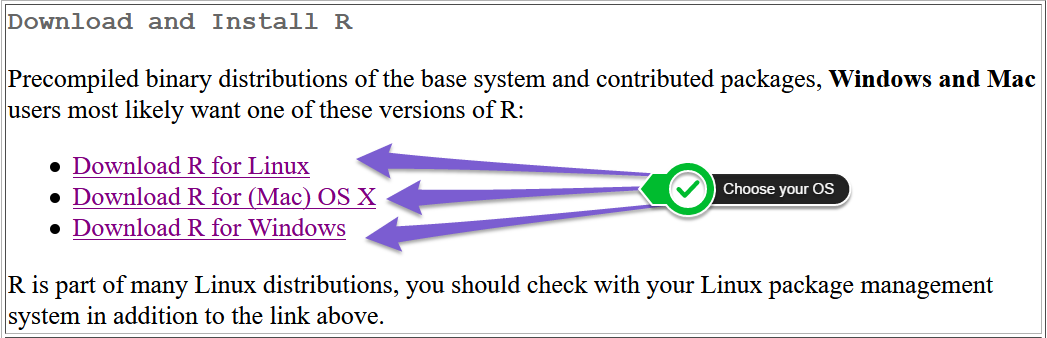
\includegraphics[width=6in]{RCranInstallImage.png}}
		
\vspace*{1em}		
		
		If you are using a Mac, then select the most recent R-3.x.x.pcg file. Open the downloaded file and follow the on-screen instructions to complete your installation.\\
		\fbox{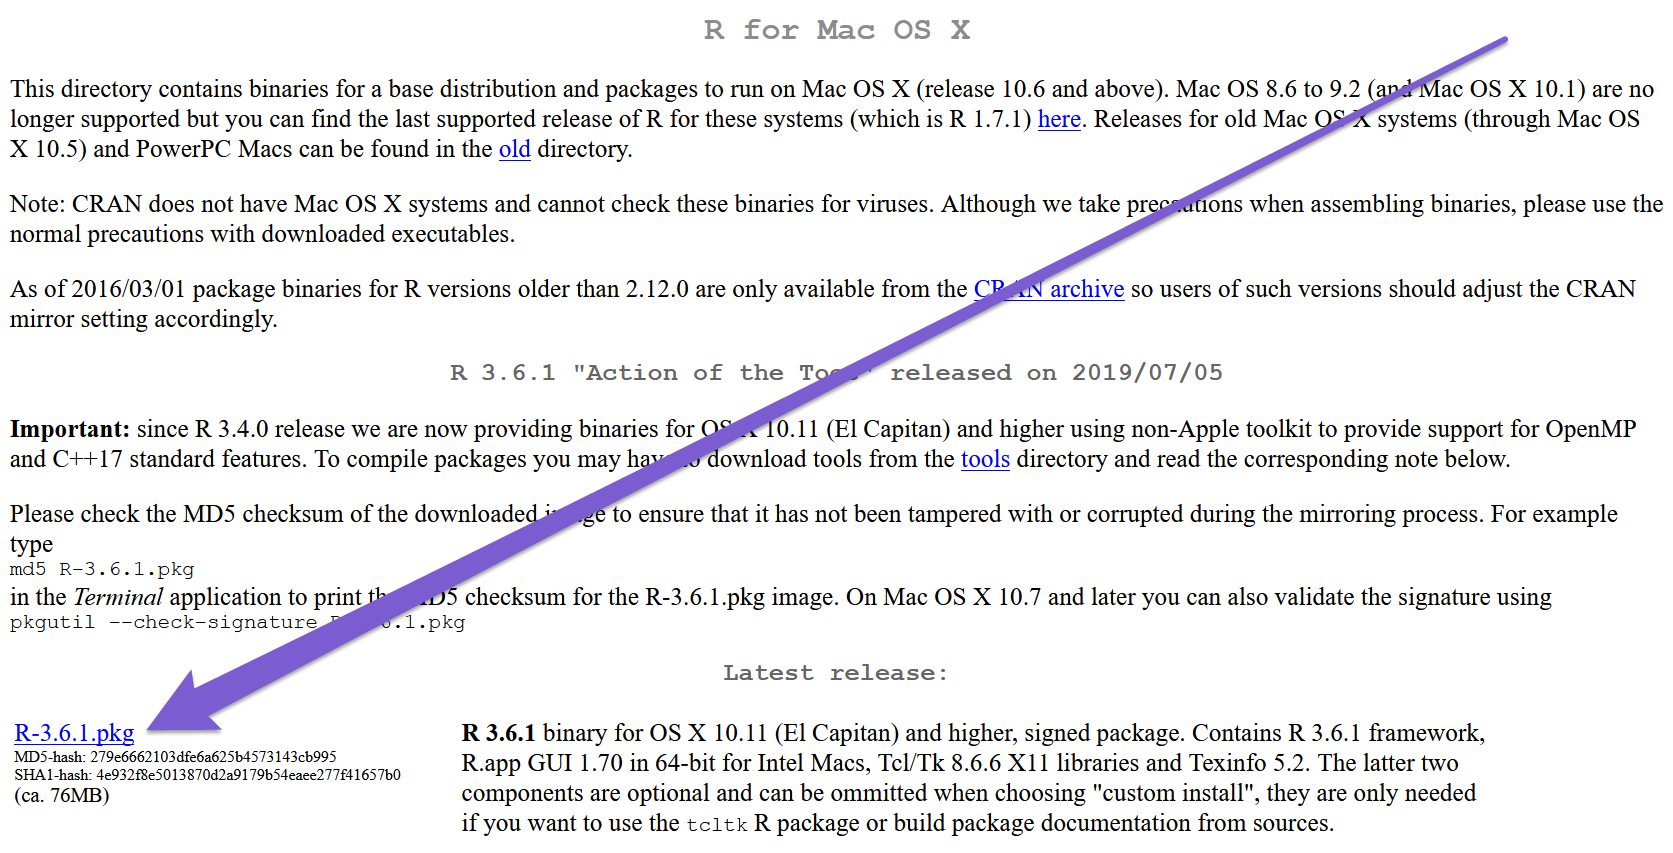
\includegraphics[width=6in]{RCranMacImage.png}}
\newpage
		If you are using Windows, then select the "base" distribution of R. Download the indicated and follow the on-screen instructions to complete your installation.\\
		\fbox{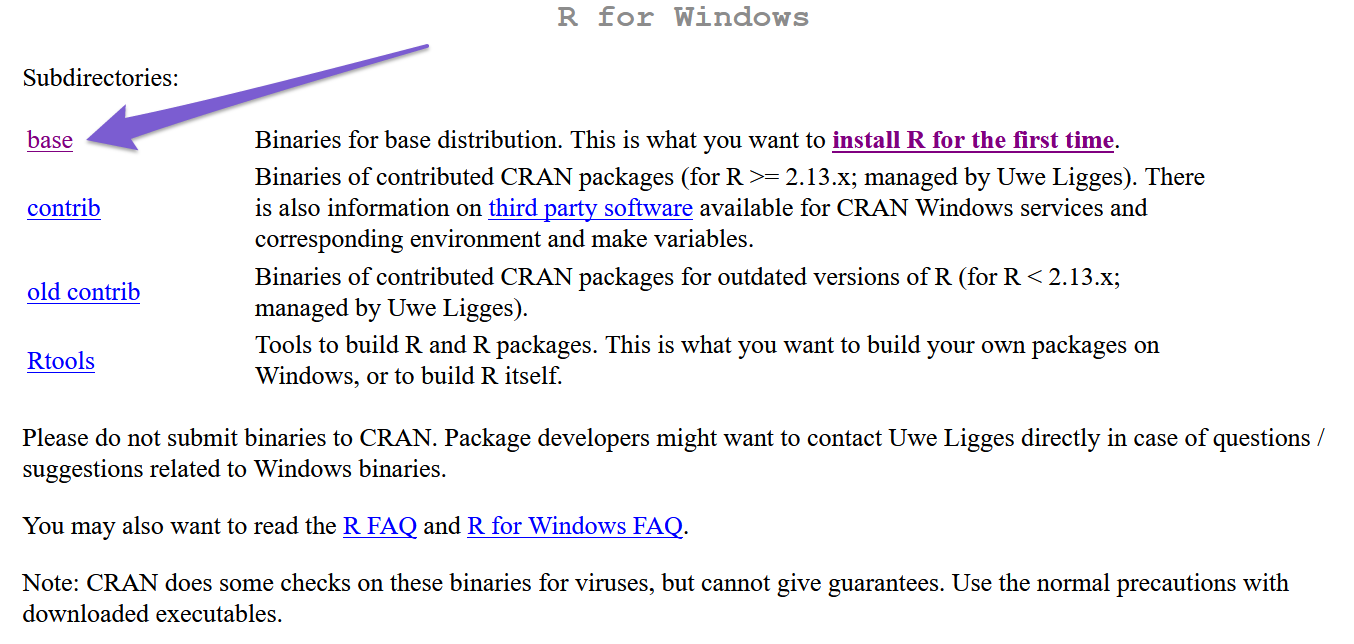
\includegraphics[width=6in]{RCranWindowsImage.png}}
		
		If you are using Linux, then select your Linux distribution. The website will provide you with the commands necessary to install R.
	
	\item \textbf{Installing R Studio:}\\ \vspace{1em}
		To install R Studio, navigate to \href{https://rstudio.com/products/rstudio/download/#download}{rstudio.com/products/rstudio/download}. Select your operating system, and follow the installer's instructions. 
		\fbox{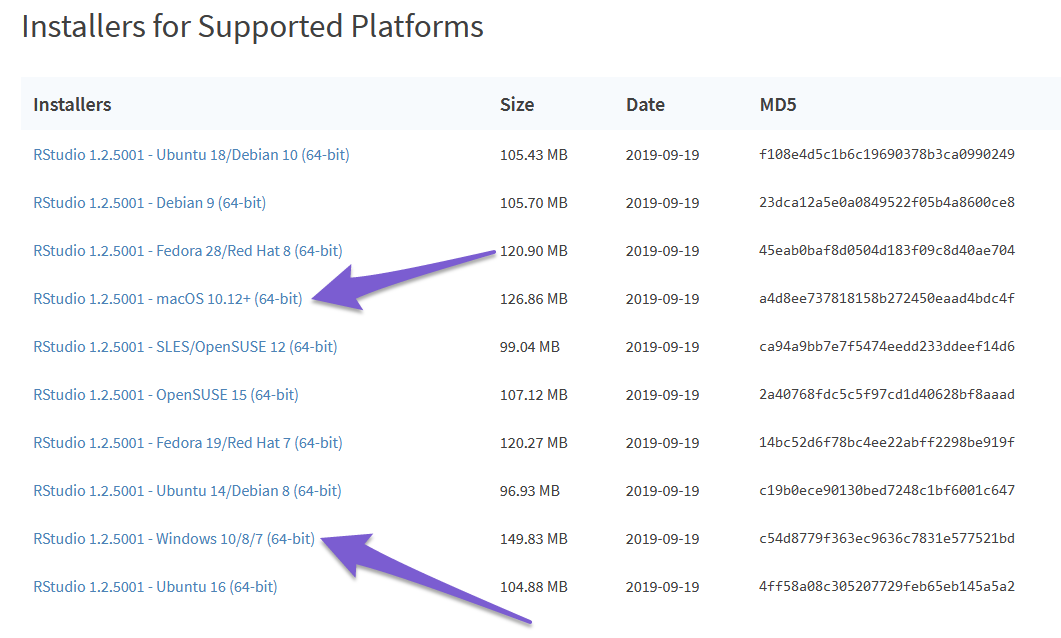
\includegraphics[width=6in]{RStudioInstall.png}}
	\item \textbf{Congratulations, you're ready to start using R Studio.}
\end{enumerate}



\newpage
\pagenumbering{arabic}




%Lab Title
\section{The Basics}

% Section 1, the R Screen
\subsection{The R Screen}
\normalsize The R Studio screen is split into \textbf{4} areas.
\begin{enumerate}
\item The Console (Bottom Left) - where you input commands and where the output is usually displayed.
\item The File Editor and Data Browser Window (Top Left) - when open, this window allows you to look at a two-dimensional, cell-based display of your data and edit special R files.
\item The Environment \& History Window (Top Right) - provides a list of objects (like datasets) currently loaded and usable in the Environment tab, and a history of all the commands you typed in in the History tab.
\item The Utility Tab (Bottom Right) - provides a list of files you can open in the Files tab, displays plots and graphs in the Plots tab, shows a list of currently installed packages in the Packages tab, and finally shows help documentation in the Help tab.
\end{enumerate}

% Section 2: Loading and Browsing Data
\subsection{Loading Data into R}
\normalsize The first step to doing any data analysis in R is loading the data into R. If the data is in an R friendly file format - most commonly .Rda - then it can be opened like any other computer document. If the data is in another file format, it will need to be imported.
Note that R can have multiple datasets loaded at once.

\vspace{.5em}

\begin{tcolorbox}[title = Loading Datasets]
  For R Data (.Rda files): \\
\ind File $>$ Open $>$ Select the .rdata File \vspace{1em}\\
  For Other Data Files (e.g. .xlsx, .csv, .dta):\\
\ind  File $>$ Import $>$ From File Type \\
\ind  Browse and Select File \\
\ind  Make Sure to Give Your Dataset a Name! (You'll be typing it a lot!) 
\end{tcolorbox}

% Section 3, Interacting with Data
\subsection{Viewing and Editing Data in R}
The second step of doing data analysis in R is viewing and sorting your data.

\vspace{.5em}

\begin{tcolorbox}[title = Basic Data Viewing and Editing]
To browse your dataset like a spreadsheet: (Make sure to use a capital \textbf{V}!)
\begin{lstlisting}
  View(`\textit{datasetName}`)
\end{lstlisting}
\end{tcolorbox}


\begin{tcolorbox}[title = Basic Data Viewing and Editing (cont.)]
Typically, when referring to a variable in a command you must refer to the dataset the variable is in as follows:
\begin{lstlisting}
  `\textit{datasetName}`$`\textit{variableName}`
\end{lstlisting}
Sorting can be useful to look for common categories when creating a table. To sort your data by a variable: 
\begin{lstlisting}
  sort(`\textit{datasetName}`$`\textit{variableName}`)
\end{lstlisting}
If you "attach" a dataset, R will assume that you're always referencing variables in that dataset: an optional but big time saver. To attach a dataset:
\begin{lstlisting}
  attach(`\textit{datasetName}`)
\end{lstlisting}
\end{tcolorbox}


% Section 4, Viewing Summaries
\subsection{Viewing Summaries of the Data}
The third step of doing data analysis is looking at some basic statistical attributes of your data and your variables.
\begin{tcolorbox}[title = Viewing Data Summaries]
To view a list of all variables in your dataset:
\begin{lstlisting}
  names(`\textit{datasetName}`)
\end{lstlisting}
To view the basic structure of all variables in your dataset:
\begin{lstlisting}
  str(`\textit{datasetName}`)
\end{lstlisting}
To view a basic summary of a variable (e.g. Mean, Median, Min, Max):
\begin{lstlisting}
  summary(`\textit{datasetName}`$`\textit{variableName}`)
\end{lstlisting}
To view more a more detailed summary of a variable (e.g. N, SD, Kurtosis)
\begin{lstlisting}[frameround = t t t t, backgroundcolor = \color{lightgray}]
  install.packages("`\textit{psych}`")
\end{lstlisting}
\begin{lstlisting}
  library(`\textit{psych}`) `\vspace{-.5em}`
`\rule{\textwidth}{0.2pt}`
  describe(`\textit{datasetName}`$`\textit{variableName}`)
\end{lstlisting}
To view a cross-tabulation of a nominal or ordinal variable:
\begin{lstlisting}
  table(`\textit{datasetName}`$`\textit{variableName}`)
\end{lstlisting}
\end{tcolorbox}
\begin{tcolorbox}[title = Viewing Data Summaries (cont.)]
Or for an easier-to-read cross-tab:
\begin{lstlisting}[frameround = t t t t, backgroundcolor = \color{lightgray}]
  install.packages("`\textit{gmodels}`")
\end{lstlisting}
\begin{lstlisting}
  library(`\textit{gmodels}`) `\vspace{-.5em}`
`\rule{\textwidth}{0.2pt}`
  CrossTable(`\textit{datasetName}`$`\textit{variableName}`)
\end{lstlisting}
\end{tcolorbox}

% Section 5, Creating and Recoding Variables
\subsection{Creating and Editing Variables}
\normalsize 
A large part of data analysis is being able to generate and recode variables from an existing dataset or even data you've collected yourself. Many of the commands in this section rely on the \textit{dplyr} package, which provides easier ways to manipulate variables in your dataset. 

\vspace{1em}

\begin{tcolorbox}[title = Recoding Variables]
Before proceeding, make sure you have the \textit{tidyverse} package installed and loaded. Installing the \textit{tidyverse} collection of packages includes \textit{dplyr} and a number of other useful tools we will use later on. 
\begin{lstlisting}[frameround = t t t t, backgroundcolor = \color{lightgray}]
  install.packages("`\textit{tidyverse}`")
\end{lstlisting}
Once installed, we need to load the \textit{tidyverse} package set to use it. \\ \ind We do this with a library() command.
\begin{lstlisting}
  library(`\textit{tidyverse}`)
\end{lstlisting}
To create a variable by applying mathematical functions to other variables:\\
\ind The example here is addition, but you could also subtract, multiply and divide. 
\begin{lstlisting}
`\textit{dataset}` <-
    mutate(`\textit{dataset}`, `\textit{newVariable}` = `\textit{oldVariable1}` + `\textit{oldVariable2}`)
\end{lstlisting}
To recode a variable:\\
\ind Recoding a variable involves altering the values of an existing variable and placing them into a new variable. For example, your data may have a variable for an individual's party membership. You may only care about membership in one party, so you would recode the party variable from having 15 values to only being a 0 or a 1. 0 for non-members of "Imaginary Party" and 1 for members.
\begin{lstlisting}
`\textit{dataset}` <-
    mutate(`\textit{dataset}`, 
        `\textit{newVariable}` = case_when(`\textit{oldVar}` == `\textit{oldVal1}` ~ `\textit{newVal1}`,
  	                      `\textit{oldVar}` != `\textit{oldVal2}` ~ `\textit{newVal2}`))
\end{lstlisting}
\end{tcolorbox}
\begin{tcolorbox}[title = Recoding Variables (cont.)]
mutate() creates a new variable based on an argument given to it.\\
case\_when() provides an argument for mutate() which sets the New Variable equal \\ \ind to newVal1 if the Old Variable was equal to oldVal1, and newVal2 if the Old \\ \ind Variable was equal to oldVal2.\\
Note that the symbol between the oldVal and newVal is a tilde, typically the Shift + ` \\ \ind option on most keyboards, found above the Tab key.\\
$!=$ is interpreted to mean "not equal to" by \textit{R}.\\
\vspace{.5em}

Recoding as a dummy:\\
\ind Alternatively, we could recode a variable with many different categories into a dichotomous variable. The below example turns a variable with five categories into a dichotomous variable where the first category becomes one while the rest become zero. If we do not include a value in the mutate command and do not specify a new category using a logic of the original variable being greater than, less than, or not equal to a value; then the resulting new variable will treat unspecified values as missing. This is important if we want to exclude certain values from our analysis, say negative numbers or exceptionally large values which some datasets use to communicate reasons for missingness.
\begin{lstlisting}
`\textit{dataset}` <-
    mutate(`\textit{dataset}`, 
        `\textit{newVariable}` = case_when(`\textit{oldVar}` == `\textit{oldVal1}` ~ `1`,
  	                      `\textit{oldVar}` == `\textit{oldVal2}` ~ 0,
  	                      `\textit{oldVar}` == `\textit{oldVal3}` ~ 0,
  	                      `\textit{oldVar}` == `\textit{oldVal4}` ~ 0,
  	                      `\textit{oldVar}` == `\textit{oldVal5}` ~ 0))
\end{lstlisting}
So if the above command were run, but it actually had a sixth category where -9 represents respondents who refuse to answer; those -9's would become \textit{NA}'s, R's representation for missing data. If we recoded using \textit{oldVar =! 1}, then the -9's would become zeros. We can visualize this below. \vspace{.5em} 

Specifying each category (1 through 5) separately:\\
\begin{center}
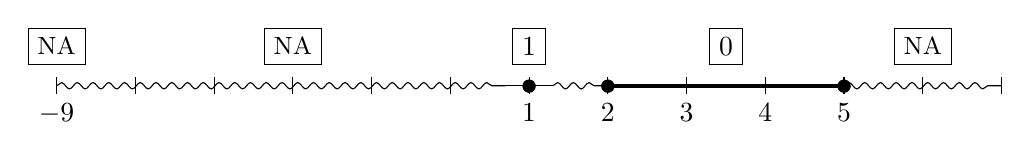
\begin{tikzpicture}
    \draw [-,decorate,decoration={snake,amplitude=.4mm,segment length=2mm,post length=1mm}] (-5,0) -- (.7,0);
    \draw (.7,0) -- (1.3,0);
    \draw[-,decorate,decoration={snake,amplitude=.4mm,segment length=2mm,post length=1mm}] (1.3,0) -- (2,0);
    \draw (2,0) -- (5,0);
    \draw[-,decorate,decoration={snake,amplitude=.4mm,segment length=2mm,post length=1mm}] (5,0) -- (7,0);
	\node at (1,.5) [shape=rectangle,draw] {1}; 
	\node at (3.5,.5) [shape=rectangle,draw] {0};
	\node at (-5,.5) [shape=rectangle,draw] {\small{NA}};
	\node at (-2,.5) [shape=rectangle,draw] {\small{NA}};
	\node at (6,.5) [shape=rectangle,draw] {\small{NA}};
	\foreach \x in  {-5,-4,-3,-2,-1,0,1,2,3,4,5,6,7} % edit here for the vertical lines
	\draw[shift={(\x,0)},color=black] (0pt,3pt) -- (0pt,-3pt);
	\foreach \x in {1,2,3,4,5} % edit here for the numbers	
	\draw[shift={(\x,0)},color=black] (0pt,0pt) -- (0pt,-3pt) node[below] {$\x$};
	\draw[shift={(-5,0)},color=black] (0pt,0pt) -- (0pt,-3pt) node[below] {$-9$};
	\draw[*-o] (2,.078);
	\draw[*-o] (5,.078);
	\draw[ultra thick] (1.92,0) -- (4.92,0);
	\draw[*-o] (1,.078);
\end{tikzpicture}
\end{center}
\vspace{.5em}

Using not-equal to ($!=$):
\begin{center}
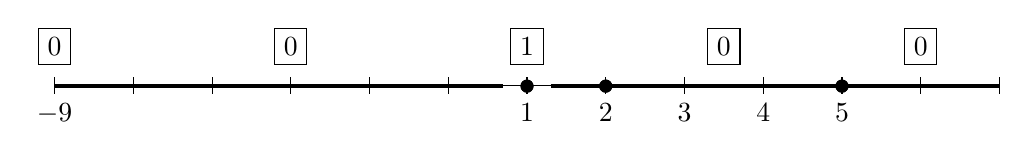
\begin{tikzpicture}
    \draw (-5,0) -- (.7,0);
    \draw (.7,0) -- (1.3,0);
    \draw (1.3,0) -- (2,0);
    \draw (2,0) -- (5,0);
    \draw (5,0) -- (7,0);
	\node at (1,.5) [shape=rectangle,draw] {1}; 
	\node at (3.5,.5) [shape=rectangle,draw] {0};
	\node at (-5,.5) [shape=rectangle,draw] {0};
	\node at (-2,.5) [shape=rectangle,draw] {0};
	\node at (6,.5) [shape=rectangle,draw] {0};
	\foreach \x in  {-5,-4,-3,-2,-1,0,1,2,3,4,5,6,7} % edit here for the vertical lines
	\draw[shift={(\x,0)},color=black] (0pt,3pt) -- (0pt,-3pt);
	\foreach \x in {1,2,3,4,5} % edit here for the numbers	
	\draw[shift={(\x,0)},color=black] (0pt,0pt) -- (0pt,-3pt) node[below] {$\x$};
	\draw[shift={(-5,0)},color=black] (0pt,0pt) -- (0pt,-3pt) node[below] {$-9$};
	\draw[*-o] (2,.078);
	\draw[*-o] (5,.078);
	\draw[ultra thick] (1.3,0) -- (4.92,0);
	\draw[ultra thick] (-5,0) -- (0.7,0);
	\draw[ultra thick] (5,0) -- (7,0);
	\draw[*-o] (1,.078);
\end{tikzpicture}
\end{center}
\end{tcolorbox}

% Other Tips!
\subsection{Some Final Tips on Packages, Finding Help in R, and Keyboard Shortcuts}

\vspace{1em}

\begin{tcolorbox}[title = Packages]
Packages are sets of useful commands that R does not include by default. \\
If we show a command that requires a library() command, then the command needs a package installed and loaded to work!\vspace{1em}\\
First, you need to install the package. This only needs to be done once per computer.
\begin{lstlisting}[frameround = t t t t, backgroundcolor = \color{lightgray}]
  install.packages("`\textit{packageName}`")
\end{lstlisting}
Then load the package so we can use the commands! This needs to be done once per session.
\begin{lstlisting}
  library(`\textit{packageName}`)
\end{lstlisting}
Now we can access all of the commands included in the package!
\end{tcolorbox}

\begin{tcolorbox}[title = Help!]
If you need any help with a command, try ...
\begin{lstlisting}
  ?`\textit{commandName}`
\end{lstlisting}
... and R Studio will open the documentation for the command.
\\
As always, Google can be a great resource too if you're looking for how to use a command or do something in R!
\end{tcolorbox}

\begin{tcolorbox}[title = Shortcuts!]
When typing in commands, variables, or datasets into R Studio's Command Window a list will pop-up, showing terms that may complete what you're typing. Hitting TAB will insert R Studio's current suggested command or variable. This means you only have to type out a little bit of the term into the console, and R Studio can fill in the rest!\\
For example typing...
\begin{lstlisting}
  summ
\end{lstlisting}
and hitting TAB... will produce
\begin{lstlisting}
  summary(|)
\end{lstlisting}
with the cursor ready to fill in the parentheses!
\end{tcolorbox}

\subsection{Using R-Scripts (with Example Script)}
\normalsize
% Section 2, R Scripts
\begin{tcolorbox}[title = R Scripts]

An R script is a file containing a set of R commands.\vspace{.5em}\\
R scripts are therefore great for keeping track of and replicating all of the commands\\ \ind you may have used to get your results. \vspace{.5em}\\ 
To create an R script in RStudio:
\begin{lstlisting}
  File > New File > R Script
\end{lstlisting}
The R Script should open in the upper left section of RStudio, above\\ \ind the Console section.\vspace{.5em}\\
It is a good idea to immediately save your R script on creation using:
\begin{lstlisting}
  File > Save As
\end{lstlisting}
To run a single command in the R Script: \\
\ind Place the cursor on the line you wish to run, and hit the run button at the top\\ \ind right corner of the R Script.\vspace{.5em} \\
To run every command in the R Script in order: \\ 
\ind Click the Source button at the top of the R Script.\vspace{.5em}\\
\ind Alternatively, click the "Source on Save" box at the top of the R script, then\\ \ind click on the Floppy Disk save symbol. This will save the R Script \textit{and} run every\\ \ind command in the R Script.
\end{tcolorbox}

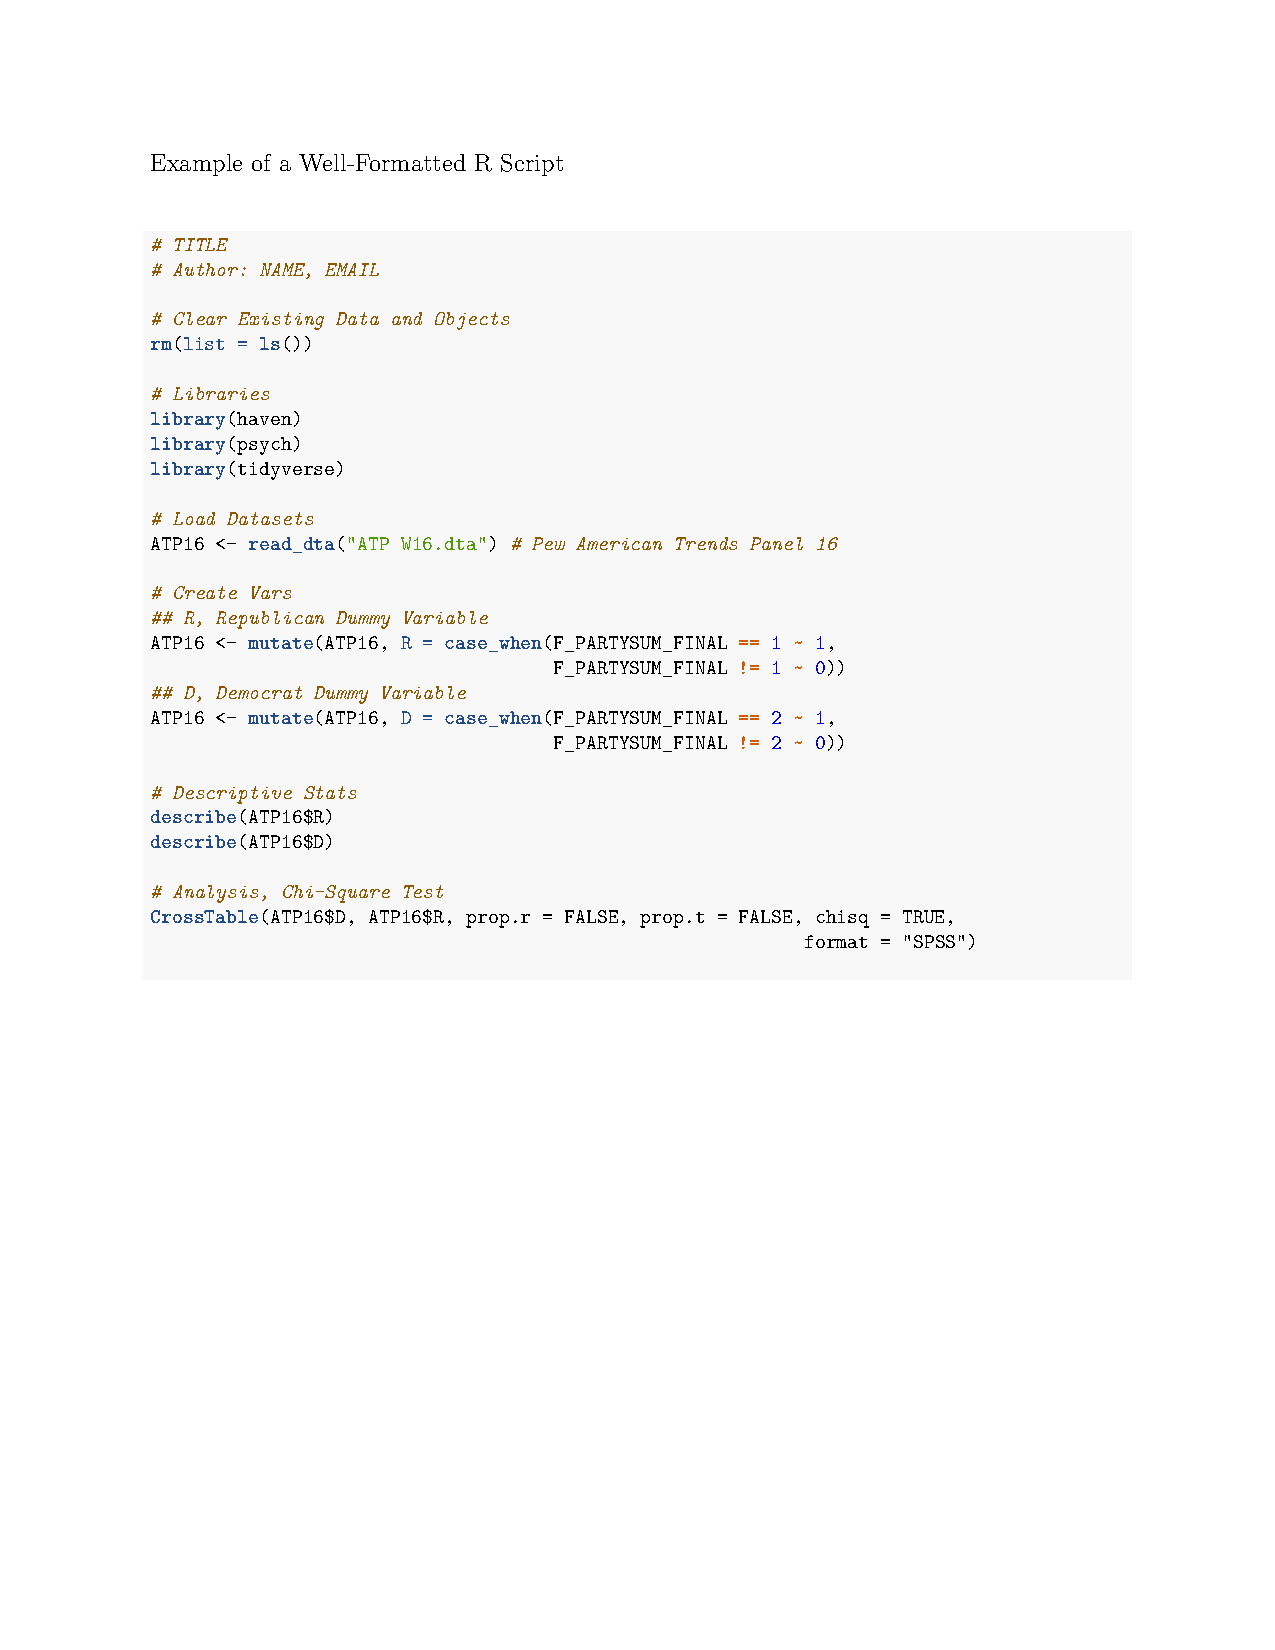
\includepdf{Example-RScript.pdf}
\normalsize 


%%%%%%%%%
% Lab 2: Descriptives and Bivariate Hyp. Testing
\section{Descriptive Stats and Bivariate Hypothesis Testing}

\vspace{1em}

% Section 1, Basic Descriptives
\subsection{Descriptive Statistics}

We seek descriptive statistics to understand the basic attributes of our data and variables. Typically, descriptive statistics involve commonly understood stats such as the mean, median, range and standard deviation. In some specific case, descriptive statistics can also include the interquartile range, skew and kurtosis.

\normalsize
\begin{tcolorbox}[title = Descriptive Statistics]
Finding the mean, median, minimum, maximum and inter-quartile range:
\begin{lstlisting}
  summary(`\textit{dataset\$varName}`)
\end{lstlisting}
Finding the N, standard deviation, range, skew and kurtosis:
\begin{lstlisting}
  library(psych) `\vspace{-.5em}`
`\rule{\textwidth}{0.2pt}`
  describe(`\textit{dataset\$varName}`)
\end{lstlisting}
Finding the mode:\\
\ind Hint: Look for the value that occurs most in the table.
\begin{lstlisting}
  table(`\textit{dataset\$varName}`)
\end{lstlisting}

\end{tcolorbox}

% Section 3, Subsetting Data
\subsection{Subsetting Data}

Subsetting data is an \textit{incredibly} common tool we use when performing data management and analysis. By subsetting data, we mean selecting a portion of the data - hence \textit{subset}ing - in order to understand or alter it. For example, maybe we wish to know the mean education levels for only one sex. We would select a subset of the data where only men or women are included, to find the mean education level of only those men or women.

\begin{tcolorbox}[title = Subsetting Data]

Select \textit{Variable 1} when \textit{Variable 2} is \textit{equal to} a given \textit{value}*
\begin{lstlisting}
  `\textit{dataset\$var1}`[`\textit{dataset\$var2}` == `\textit{value}`]
\end{lstlisting}

Select \textit{Variable 1} when \textit{Variable 2} is \textit{\textbf{not} equal to} a given \textit{value}*
\begin{lstlisting}
  `\textit{dataset\$var1}`[`\textit{dataset\$var2}` != `\textit{value}`]
\end{lstlisting}

Select \textit{Variable 1} when \textit{Variable 2} is \textit{greater than} a given \textit{value}* \\
\ind \small{(use \textit{$>=$} for \textit{greater than or equal to)}}
\begin{lstlisting}
  `\textit{dataset\$var1}`[`\textit{dataset\$var2}` > `\textit{value}`]
\end{lstlisting}
\end{tcolorbox}

\begin{tcolorbox}[title = Subsetting Data (cont.)]

Select \textit{Variable 1} when \textit{Variable 2} is \textit{less than} a given \textit{value}* \\
\ind \small{(use \textit{$<=$} for \textit{less than or equal to)}}
\begin{lstlisting}
  `\textit{dataset\$var1}`[`\textit{dataset\$var2}` < `\textit{value}`]
\end{lstlisting}

Example: Means of Income for Men and Women
\begin{lstlisting}
  mean(anes2016$income[anes2016$sex == 1])
  mean(anes2016$income[anes2016$sex == 0])
\end{lstlisting}

\vspace{1em}

\small{* Note that \textit{Variable 2} can also be \textit{Variable 1}, so the below is a valid command.}
\begin{lstlisting}
  mean(anes2016$income[anes2016$income >= 1])
\end{lstlisting}

\end{tcolorbox}


\subsection{Recoding Using Subsetting}
In cases where you want to make alterations to an existing variable, it is sometimes useful to make a quick recode with using R's subset functionalities. This is especially useful for recoding values to be missing (aka null).
\begin{tcolorbox}[title = Recoding Using Subset Brackets]
\begin{lstlisting}
 `\textit{dataset\$variable}`[`\textit{dataset\$variable}` == `\textit{value}`] <- NA
 `\textit{dataset\$variable}`[`\textit{dataset\$variable}` <  `\textit{value}`] <- NA
 `\textit{dataset\$variable}`[`\textit{dataset\$variable}` <= `\textit{value}`] <- NA
 `\textit{dataset\$variable}`[`\textit{dataset\$variable}` >  `\textit{value}`] <- NA
 `\textit{dataset\$variable}`[`\textit{dataset\$variable}` >= `\textit{value}`] <- NA
 `\textit{dataset\$variable}`[`\textit{dataset\$variable}` != `\textit{value}`] <- NA
\end{lstlisting}
Note that you could recode as missing if a variable is:\\
\ind equal to ($==$) a value\\
\ind greater than ($>$); or greater than or equal to ($>=$) a value\\
\ind less than ($<$); or less than or equal to ($<=$) a value\\
\ind not equal to ($!=$) a value
\end{tcolorbox}

% Section 2, Chi-Square 
\subsection{Chi-Square Test (Categorical X by Categorical Y)}
A Chi-Square test is used to test for a correlation between a Categorical Independent Variable and a Categorical Dependent Variable.
\begin{tcolorbox}[title = Chi-Square Test (Categorical X by Categorical Y)]
Chi-Square Table:
\begin{lstlisting}[frameround = t t t t, backgroundcolor = \color{lightgray}]
  install.packages("`\textit{descr}`")
\end{lstlisting}
\begin{lstlisting}
  library(descr) `\vspace{-.5em}`
`\rule{\textwidth}{0.2pt}`
  CrossTable(`\textit{dataset\$varY}`, `\textit{dataset\$varX}`, prop.t = FALSE, chisq = TRUE,
                                                   format = "SPSS")
\end{lstlisting}
Basic Interpretation:\\
\ind Use the p-value of the Pearson's Chi-squared Test to understand if the \\ \ind \ind  relationship between X and Y is statistically significant.\\
\ind Use the cross-tabulation to interpret the direction of the relationship. 
\end{tcolorbox}

% Section 3, t-test
\subsection{T-Test (Dichotomous X by Continuous Y)}
A T-Test is used to test for a correlation between a Dichotomous Independent Variable and a Continuous Dependent Variable.
\begin{tcolorbox}[title = T-Test (Dichotomous X by Continuous Y)]
Student's T-Test:
\begin{lstlisting}
  t.test(`\textit{dataset\$varY} $\sim$ \textit{dataset\$varX}`, var.equal = TRUE)
\end{lstlisting}
Basic Interpretation:\\
\ind Use the p-value to determine the statistical significance of the relationship \\ \ind \ind between X and Y.\\
\ind Look at which group mean is lower, that group has a significantly lower \\ \ind \ind in Y than the other group and vice versa.
\end{tcolorbox}

\vspace{-.75em}

% Section 4, Correlations
\subsection{Correlations (Continuous X by Continuous Y)}
A correlation test is specifically used to determine whether a Continuous Independent Variable and Continuous Dependent Variable are, well, correlated.
\begin{tcolorbox}[title = Correlations (Continuous X by Continuous Y)]
Basic Correlation between X and Y:
\begin{lstlisting}
  cor.test(`\textit{dataset\$varY}`, `\textit{dataset\$varX}`, method = "pearson", 
	  				     use = "complete.obs")
\end{lstlisting}
\end{tcolorbox}
\begin{tcolorbox}[title = Correlations (Continuous X by Continuous Y)(cont.)]
Basic Interpretation: \\
\ind If the p-value is less than 0.05, then the relationship between continuous variables \ind \ind X and Y is statistically significant.\\
\ind Under "sample estimates ... cor" is the correlational coefficient. This number \ind \ind tells us the resulting change in Y for a 1 unit increase in X.
\end{tcolorbox}

\vspace{-.75em}

\subsection{Correlation Tables}
Sometimes, we may want to look at the correlations between multiple variables. This will be especially useful when checking for multicollinearity later on when we are using regressions. In this example, we have three variables. However, you could use as many as you desire!
\begin{tcolorbox}[title = Correlation Table]
\begin{lstlisting}[frameround = t t t t, backgroundcolor = \color{lightgray}]
  install.packages("`\textit{Hmisc}`")
\end{lstlisting}
\begin{lstlisting}
  library(Hmisc) `\vspace{-.5em}`
`\rule{\textwidth}{0.2pt}`
  rcorr(cbind(`\textit{dataset\$varY}`,`\textit{dataset\$varX}`,`\textit{dataset\$varZ}`))
\end{lstlisting}
Basic Interpretation:\\
\ind \emph{rcorr()} produces three cross-tables (or a table for each variable provided).\\
\ind The first reports the correlational coefficient for each pair of variables. \\ 
\ind The second reports the n after excluding missing observations for the pair of \ind \ind variables. \\ 
\ind The third reports the p-values for the relationship between each pair of variables.
\end{tcolorbox}


\newpage

\section{Bivariate Regressions, Plotting, and Paper-Ready Tables}

% Section 3, Checking for Normalcy
\subsection{Checking for Normal Distributions}
When running correlations or regressions, it is important to check to see if your data is "normal". 
\begin{tcolorbox}[title = Checking for Normalcy]
The best way to check, is to look at the histogram for each variable you will be \ind correlating or regressing.
Simple Histogram:
\begin{lstlisting}
  hist(`\textit{datasetName\$varName}`)
\end{lstlisting}
\end{tcolorbox}
\begin{tcolorbox}[title = Checking for Normalcy (cont.)]

Nicer Histogram with a Normal Curve for Reference:
\begin{lstlisting}
 library(tidyverse) `\vspace{-.5em}`
`\rule{\textwidth}{0.2pt}`
 ggplot(`\textit{datasetName}`, aes(`\textit{varName}`)) +
   geom_histogram(binwidth = `\textit{2}`,
      color = "black",
      aes(y = ..density.., fill = ..count..)) +
   stat_function(fun = dnorm,
      color = "`\textit{blue}`",
      args = list(
        mean = mean(`\textit{datasetName\$varName}`[!is.na(`\textit{datasetName\$varName}`)]),
        sd = sd(`\textit{datasetName\$varName}`[!is.na(`\textit{datasetName\$varName}`)]) ) )
\end{lstlisting}
\end{tcolorbox}

\subsection{Plotting a Line of Best Fit}
\begin{tcolorbox}[title = Plotting Lines of Best Fit]
Plotting a Line of Best Fit:
\begin{lstlisting}
 library(tidyverse) `\vspace{-.5em}`
`\rule{\textwidth}{0.2pt}`
 ggplot(`\textit{dataset}`, aes(x = `\textit{varX}`, y = `\textit{varY}`)) + 
    geom_point() + 
    geom_smooth(method = lm)
\end{lstlisting}
\end{tcolorbox}

% Section 5, Bivariate OLS Regression
\subsection{Bivariate OLS Regression (Any X, Continuous Y)}
Also referred to as a bivariate linear regression, this regression checks to see if one independent variable - of any type and properly prepared - leads to a significant change in a \textit{continuous} dependent variable.
\begin{tcolorbox}[title = OLS Regression]
Bivariate Linear Ordinary Least Squares Regression:
\begin{lstlisting}
  `\textit{modelName}` <- lm(`\textit{dependentVar}` `$\sim$` `\textit{independentVar}`, data = `\textit{datasetName}`) 
  summary(`\textit{modelName}`)
\end{lstlisting}
Interpretation:\\
\ind The p-value should be at the end of the output, and if p $<$ 0.05, then the \\ \ind relationship is significant.\\
\ind The Estimate of X represents the change in Y for each 1 unit increase in X.
\end{tcolorbox}


\subsection{Paper-Ready Tables}

One issue with the output and results offered up by R is that they are - well - quite \textit{unsightly}. One would hope to never gaze upon raw results in an actual paper. As such, transforming our statistics and results into tables - and later graphs - which are ready to be put directly into a paper is a key skill. Below are the necessary commands to:

\begin{tcolorbox}[title = Paper-Ready Tables]
Remember to install Stargazer before beginning to use it:
\begin{lstlisting}[frameround = t t t t, backgroundcolor = \color{lightgray}]
  install.packages("`\textit{stargazer}`")
\end{lstlisting}
Summary Statistics:
\begin{lstlisting}
 library(stargazer) `\vspace{-.5em}`
`\rule{\textwidth}{0.2pt}`
 stargazer(as.data.frame(`\textit{dataset}`[c("`\textit{var1}`", "`\textit{var2}`")]), type = "text")
\end{lstlisting}
	  Note: You can use more than 2 variables by adding a comma and another variable.
\vspace{1.2em}\\
Regression Table:
\begin{lstlisting}
 library(stargazer) `\vspace{-.5em}`
`\rule{\textwidth}{0.2pt}`
 `\textit{model1}` <- lm(`\textit{dependentVar}` `$\sim$` `\textit{independentVar}`, data = `\textit{datasetName}`)
 `\textit{model2}` <- lm(`\textit{dependentVar}` `$\sim$` `\textit{independentVar}`, data = `\textit{datasetName}`)
 stargazer(`\textit{model1}`, `\textit{model2}`, type = "text")
\end{lstlisting}
\vspace{.5em} 
\end{tcolorbox}
\begin{tcolorbox}[title = Paper-Ready Tables Example (cont.)]
Example with Variable Labels:
\begin{lstlisting}
 model1 <- lm(conTherm `$\sim$` libTherm, data = anes_timeseries_2016)
 stargazer(model1, 
       dep.var.labels = "`Conservative Feeling Thermometer`", 
       covariate.labels = c("`Liberal Thermometer`"), type = "text")
\end{lstlisting}
Example Output:
\begin{lstlisting}
 ====================================================
                           Dependent variable:       
                     --------------------------------
                     Conservative Feeling Thermometer
 ----------------------------------------------------
 Liberal Thermometer            -0.413***            
                                 (0.014)             
                                                     
 Constant                       77.470***            
                                 (0.821)             
                                                     
 ----------------------------------------------------
 Observations                     3,566              
 R2                               0.193              
 Adjusted R2                      0.192              
 Residual Std. Error        22.415 (df = 3564)       
 F Statistic            850.692*** (df = 1; 3564)    
 ====================================================
 Note:                    *p<0.1; **p<0.05; ***p<0.01
\end{lstlisting}
Note: You can Copy + Paste this table into Word!\\
\ind Just make sure the table is formatted as Lucida Console, 10pt font.\vspace{1em} \\ 
Additional Note: If you have more the one covariate, simply add a comma after the\\ \ind first label and add the label for the next variable. The labels \textit{must} be placed in\\ \ind the same order the variables are listed in the lm() command.\vspace{.5em} \\
Example:
\begin{lstlisting}
  model1 <- lm(conTherm `$\sim$` libTherm + age,  
                                       data = anes_timeseries_2016)
 stargazer(model1, 
       dep.var.labels = "`Conservative Feeling Thermometer`", 
       covariate.labels = c("`Liberal Thermometer`", "Age"), 
       type = "text")
\end{lstlisting}
\end{tcolorbox}

% New Page
\newpage

\section{Multiple Regressions and Coefficient Plots}

\subsection{Multiple Regression (Any X, Continuous Y, Many Z)}
A multiple linear regression attempts to predict a dependent continuous variable using an independent variable of interest \textit{while} controlling for other variables.
\begin{tcolorbox}[title = Multiple Regression]
Multiple Regression Command:
\begin{lstlisting}
 `\textit{modelName}` <- lm(`\textit{depVar}` `$\sim$` `\textit{indVar\textsubscript{1}}` + `\textit{indVar\textsubscript{2}}` ... `\textit{indVar\textsubscript{n}}`, `data = \textit{dataset}`)
\end{lstlisting}
Viewing the Results:
\begin{lstlisting}
 summary(`\textit{modelName}`)
\end{lstlisting}
Interpreting the Results:\\
\ind Is the p-value of the model significant? If so, then look at the p-values for each \\ \ind \ind variable.\\
\ind If the p-value of a variable is significant, then that variable is significantly related\\ \ind \ind to the dependent variable. \\
\ind Then look at the independent variable's estimate to see the amount the \\ \ind \ind dependent variable will change based on a 1-value increase in the\\ \ind \ind independent variable.\\
Remember, you can use stargazer() to view the results as well, and use it to paste your\\ \ind  results into your paper! See Lab 3 for more on using Stargazer.
\begin{lstlisting}
 library(stargazer) `\vspace{-.5em}`
`\rule{\textwidth}{0.2pt}`
 stargazer(`\textit{modelName}`, type = "text")
\end{lstlisting}
\end{tcolorbox}

\subsection{Prepping Categorical Variables for Multiple Regression}

R needs to know a variable is categorical (with more than 2 categories) before it is entered into the regression.
There are two ways of prepping categorical variables: dummy-ing and factorizing.\vspace{.5em}
\vspace{1.5em}

\emph{Dummy-ing Out Categorical Variables:}

\vspace{.5em}
Dummy-ing Out variables refers to taking a variable of multiple values, and transforming it into a set of variables each with the values 0 or 1. To do this, we will use the ifelse() command.

\vspace{.5em}
The \emph{ifelse()} command is used to create a variable that is 1 if a condition is met, and 0 if it not. In the case of the below commands, if our categorical variable (\textit{var)} is equal to a \textit{value\textsubscript{1}}, then our new dummy variable, \textit{var\textsubscript{1}} will be set equal to 1. In all other cases, this new \textit{var\textsubscript{1}} will be 0.
Repeat the \emph{ifelse()} command until every category of our original var (\textit{var}) has its own dummy variable. Just remember to exclude one category from the regression itself to act as a reference category.

\begin{tcolorbox}[title = Prepping Categorical Dependent Variables for Multiple Regression (Dummy-ing)]
\begin{lstlisting}
 `\textit{dataset\$var\textsubscript{1}}` <- ifelse(`\textit{dataset\$var}` == `\textit{value\textsubscript{1}}`, 1, 0)
 `\textit{dataset\$var\textsubscript{2}}` <- ifelse(`\textit{dataset\$var}` == `\textit{value\textsubscript{2}}`, 1, 0)
 `...`
 `\textit{dataset\$var\textsubscript{n}}` <- ifelse(`\textit{dataset\$var}` == `\textit{value\textsubscript{n}}`, 1, 0)
\end{lstlisting}
\end{tcolorbox}

\vspace{1em}
\emph{Factorizing a Categorical Variable}\\

\vspace{.5em}
Factorizing a categorical variable involves manually telling R each value of the categorical variable and what label it represents. Therefore R can then dummy-out the variable under the hood each time we use it.
\begin{tcolorbox}[title = Prepping Categorical Dependent Variables for Multiple Regression (Factorizing)]
\ind First, check to see if the variable is recognized as a categorical (factor) variable.
\begin{lstlisting}
 is.factor(`\textit{dataset\$var}`)
\end{lstlisting}
 If this command returns TRUE, you're good to go!\\
 If this command returns FALSE, you'll need to do the following:
\begin{lstlisting}
 `\textit{dataset\$var}` <- factor(`\textit{dataset\$var}`, levels = c(`\textit{0}`, `\textit{1}`,...`\textit{n}`),
                 labels = c("`\textit{label\textsubscript{1}}`", "`\textit{label\textsubscript{2}}`", ... "`\textit{label\textsubscript{n}}`"))
\end{lstlisting}
Note! \\
\ind R will use the first factor level as the reference category, so make sure to put the \\ \ind reference category you want first. The levels do not need to go in numeric order.
\end{tcolorbox}

\subsection{Coefficient Plots}
Coefficient plots allow us to visually display the sometimes overwhelming numbers created by regression.
\begin{tcolorbox}[title = Coefficient Plots]
Required Package:
\begin{lstlisting}[frameround = t t t t, backgroundcolor = \color{lightgray}]
  install.packages("`\textit{arm}`")
\end{lstlisting}
\begin{lstlisting}
 library(arm)
\end{lstlisting}
\end{tcolorbox}
\begin{tcolorbox}[title = Coefficient Plots (cont.)]
Simple Coefficient Plot:
\begin{lstlisting}
 coefplot(`\textit{modelName}`)
\end{lstlisting}
Interpreting a Coefficient Plot:\\
\ind Each dot on a coefficent plot represents the regression estimate for a given\\ \ind \ind variable. \\
\ind The lines extending from each dot represent the 95\% confidence interval\\ \ind \ind  surrounding that estimate.\\
\ind If a confidence interval crosses the 0 line, then that variable has an insignificant\\ \ind \ind  relationship with the dependent variable.\\
\ind If a confidence interval does not touch the 0 line, then that variable does have a \\ \ind \ind significant relationship with the dependent variable. \\
\ind If a independent variable is significant, then we are 95\% confident that the value \\ \ind \ind of a 1 unit increase in the variable leads to a change in the dependent\\ \ind \ind  variable equal to a value somewhere along the confidence interval line. 
\vspace{1em}\\
Advanced Coefficient Plot (including Options):
\begin{lstlisting}
coefplot(`\textit{modelName}`, 
         pch.pts = `\textit{pointShape}`, 
         frame.plot = TRUE, 
         xlim = c(`\textit{lowerBound}`, `\textit{upperBound}`), 
         col.pts = c("`\textit{color\textsubscript{1}}`", "`\textit{color\textsubscript{2}}`", ... , "`\textit{color\textsubscript{n}}`"), 
         mar = c(`\textit{bottomMargin}`, `\textit{leftMargin}`, `\textit{topMargin}`, `\textit{rightMargin}`), 
         varnames = c("`\textit{label\textsubscript{1}}`", "`\textit{label\textsubscript{2}}`", ... "`\textit{label\textsubscript{n}}`"))
\end{lstlisting}
\textit{pointshape} will change the shape of the dot on the plot (e.g. circle, square, etc)\\
\textit{lowerbound} and \textit{upperbound} alter the min and max values of the graph plane.\\
\textit{margins} set the margins around the plot. It is common to change the left margin \\ \ind if the variable names are too long (and therefore run off the screen).\\
\textit{label\textsubscript{n}} is used to label each variable according to a chosen name. The labels must be  \\ \ind in the same order as in the original \textit{lm} model, though \textit{label\textsubscript{1}} will always be \\ \ind  "Constant".
\end{tcolorbox}

\begin{tcolorbox}[title = Coefficient Plots (cont.)]
Example Plot:
\begin{lstlisting}
model.1 <- lm(TransTherm `$\sim$` FEMALE + RACE + RELIGION + AGE, 
              data = anes_timeseries_2016)
coefplot(model.1, 
         pch.pts = 0, 
         frame.plot = TRUE, 
         xlim = c(-20, 15), 
         col.pts = c("black", "blue", "red", "green", "purple", 
           "pink", "orange"), 
         mar = c(1,6,5.1,2), 
         varnames = c("Constant", "Female", "Race` - `Black", 
           "Race` - `Asian", "Race` - `Native", "Race` - `Hispanic", 
           "Race` - `Other", "Religious", "Age"))
\end{lstlisting}
\begin{center}
\includegraphics[scale=.5]{CoeffPlot.eps}
\end{center}
\end{tcolorbox}

\section{Interaction Effects and Logistic Regressions (Any X, Dummy Y, Many Z)}

\subsection{Interaction Effects}
An interaction effect is useful if you think the effect of your independent variable is contingent on the presence of another independent variable.

\vspace{.5em}

\begin{tcolorbox}[title = Interaction Effects]
Required Package:
\begin{lstlisting}
 library(tidyverse)
\end{lstlisting}
Multiple Regression with Interaction between X\textsubscript{1} and X\textsubscript{2}:
\begin{lstlisting}
 `\textit{modelName}` <- lm(`depVar` `$\sim$` `\textit{X\textsubscript{1}}` * `\textit{X\textsubscript{2}}` + `\textit{X\textsubscript{2}}` + ... `\textit{X\textsubscript{n}}`)
\end{lstlisting}
Interpretation:\\
\ind Check to see if the interaction, \textit{X\textsubscript{1}}:\textit{X\textsubscript{2}}, is significant (p $<$ .05).\\
\ind If so, the estimate of \textit{X\textsubscript{1}} is the value of \textit{X\textsubscript{1}} when \textit{X\textsubscript{2}} is zero; and vice versa.
\ind \ind Note: It might be useful to center continuous variables around the mean, so\\ \ind \ind when \textit{X\textsubscript{1}} is 0, it is at the mean.\\
\ind However, the best way to interpret a significant interaction is to graph it...
\vspace{.5em}\\
Plotting an Interaction (\textit{X\textsubscript{2}} Variable \emph{must} be Categorical):
\begin{lstlisting}
 qplot(x = `\textit{X\textsubscript{1}}`, y = `\textit{depVar}`, facets = `$\sim$``\textit{X\textsubscript{2}}`, data = na.omit(`\textit{dataset}`)) + 
    geom_smooth(method = "lm")
\end{lstlisting}
One additional way to interpret interactions is using predicted probabilities. See the\\ \ind below section on Predicted Probabilities for more info!
\end{tcolorbox}

\subsection{Logistic Regression (Any X, Dichotomous Y, Many Z)}
Logistic regressions, similar to OLS / Linear Regressions, attempt to predict a dependent variable using an independent variable \textit{while} controlling for any number of other control variables. However instead of a continuous dependent variable, logits - short for logistic regressions - work on \textit{dichotomous} dependent variables. A crucial side effect of the dependent variable being dichotomous is that it drastically complicates interpretation of the regression results.
\begin{tcolorbox}[title = Logistic Regression]
 Logistic Regression Model:
\begin{lstlisting}
 `\textit{modelName}` <- glm(`\textit{depVar}` `$\sim$` `\textit{X\textsubscript{1}}` + `\textit{X\textsubscript{2}}` + `\textit{X\textsubscript{2}}` + ... `\textit{X\textsubscript{n}}`, family = binomial, 
                  data = `\textit{dataset}`) 
 summary(`\textit{modelName}`)
\end{lstlisting}
Interpretation:\\
\ind A logistic regression tells us the contribution of each independent variable to the\\ \ind \ind likelihood that our dependent variable will be present (have a value of 1).\\
\ind If \textit{X\textsubscript{n}} is significant (p $<$ .05), then \textit{X\textsubscript{n}} significantly alters the likelihood that our\\ \ind \ind \textit{depVar} will be present.\\
\ind Unfortunately, we cannot directly interpret the coefficients of a logistic regression\\ \ind \ind like we would a linear regression. For something similar, we use odds-ratio\\ \ind \ind coefficients ...
\vspace{.5em}\\
Required Package for Odds Ratios:
\begin{lstlisting}[frameround = t t t t, backgroundcolor = \color{lightgray}]
  install.packages("`\textit{mfx}`")
\end{lstlisting}
\begin{lstlisting}
 library(mfx)
\end{lstlisting}
Odds Ratio Coefficients for Logistic Regression:
\begin{lstlisting}
 logitor(`\textit{depVar}` `$\sim$` `\textit{X\textsubscript{1}}` + `\textit{X\textsubscript{2}}` + `\textit{X\textsubscript{2}}` + ... `\textit{X\textsubscript{n}}`, data = `\textit{dataset}`)
\end{lstlisting}
Interpretation:\\
\ind Check to see if \textit{X\textsubscript{n}} is significant (p $<$ .05).\\
\ind If so, the odd-ratio is the increased likelihood of your outcome for a 1-unit increase \\ \ind \ind in\textit{X\textsubscript{n}}. \\
\ind For example, if the odds-ratio is 0.5, then the increase of \textit{X\textsubscript{n}} by 1 will correspond\\ \ind \ind  to a .5 odds that our \textit{depVar} is 1.\\
\ind However, it is often more useful to look at the predicted probabilities of the \\ \ind \ind \textit{depVar} for a given \textit{X\textsubscript{n}}...
\end{tcolorbox}

\subsection{Predicted Probabilities}
 When discussing the results of a logistic regression, it is often useful to discuss the likelihood that your binary outcome will occur when your independent and/or control variables are of a certain variable \\
 (e.g. A man, all other variables at their means, has an 87\% chance of being registered to vote while a woman has a 90\% chance.) \vspace{.5em}
\\
\begin{tcolorbox}[title = Predicted Probabilities]
Required Package:
\begin{lstlisting}[frameround = t t t t, backgroundcolor = \color{lightgray}]
  install.packages("`\textit{ggeffects}`")
\end{lstlisting}
\begin{lstlisting}
 library(ggeffects)
\end{lstlisting}
Probabilities Given a Variable, \textit{X\textsubscript{i}}, with all Other Variables at their Means*:
\begin{lstlisting}
 ggpredict(`\textit{modelName}`, terms = "`\textit{X\textsubscript{i}}`")
\end{lstlisting}{\small * If a variable is defined as a factor, R will choose the first category.} \vspace{.5em}\\
Probabilities Given a Variable, \textit{X\textsubscript{i}}, with Specified Values of Other Variables:
\begin{lstlisting}
 ggpredict(`\textit{modelName}`, terms = "`\textit{X\textsubscript{i}}`", condition = c(`\textit{X\textsubscript{1}}` = `\textit{V\textsubscript{1}}`, 
                                             `\textit{X\textsubscript{2}}` = `\textit{V\textsubscript{2}}`, ... `\textit{X\textsubscript{n}}` = `\textit{V\textsubscript{n}}`))
\end{lstlisting}
Probabilities Given Multiple Variables:
\begin{lstlisting}
 ggpredict(`\textit{modelName}`, terms = c("`\textit{X\textsubscript{i1}}`", "`\textit{X\textsubscript{i2}}`"), condition = c(`\textit{X\textsubscript{1}}` = `\textit{V\textsubscript{1}}`, 
                                             `\textit{X\textsubscript{2}}` = `\textit{V\textsubscript{2}}`, ... `\textit{X\textsubscript{n}}` = `\textit{V\textsubscript{n}}`))
\end{lstlisting}
Plotting Probabilities*: 
\begin{lstlisting}
 `\textit{objectName}` <-  ggpredict(`\textit{modelName}`, terms = "`\textit{X\textsubscript{i}}`")
 plot(`\textit{objectName}`, log.y = TRUE)
\end{lstlisting} {\small * You can use any of the other ggpredict() commands when plotting.} \vspace{.5em}\\
Notes on Interpretation of ggpredict() Commands: \\
\ind First, look at top of the output for the "x = \textit{X\textsubscript{i}}", this will tell you what x means\\ \ind \ind in the rest of the output.\\
\ind Second, look at the bottom of the output for the section on "Adjusted for:" This\\ \ind \ind tells you the values ggpredict() assumes for all of the covariates in your \\ \ind \ind model. (It will not include variables you manually specified).\\
\ind Third, look at the cross-table in the middle of the output. This tells you the\\ \ind \ind probability of your dependent variable being present for each value of \textit{X\textsubscript{i}}. \vspace{.5em}\\
You can use ggpredict() with Ordinal Logistic Regressions and Linear Regressions as \\ \ind well! Just remove \textit{log.y = TRUE} from the plot() command.
\end{tcolorbox}

\subsection{Paper-Ready Tables: Logit Edition}
While we have already covered creating paper-ready tables using stargazer, the necessity of reporting odds ratio coefficients complicates creating a paper-ready table for a logit.
\begin{tcolorbox}[title = Paper-Ready Tables: Logit Edition]
Stargazer can take your \textit{modelName} the same as it would a Regression:
\begin{lstlisting}
 stargazer(`\textit{modelName}`, type = "text")
\end{lstlisting}
However, we may want to include odds ratios and confidence intervals in our tables. \vspace{.5em}\\
Stargazer with Odds Ratios and Confidence Intervals:
\begin{lstlisting}
 OR.vector <- exp(`\textit{modelName}`$coef)
 CI.vector <- exp(confint(`\textit{modelName}`))
 p.values <- summary(`\textit{modelName}`)$coefficients[, 4]
 stargazer(`\textit{modelName}`, coef = list(OR.vector), ci = TRUE, 
          ci.custom = list(CI.vector), p = list(p.values), 
          type = "text")
\end{lstlisting}
\end{tcolorbox}

\subsection{Ordinal Logistic Regressions}
An ordinal logistic regression is a version of a logistic regression for ordinal (rather than dichotomous) variables.\vspace{.5em}\\

\begin{tcolorbox}[title = Ordinal Logistic Regressions]
Required Package:
\begin{lstlisting}[frameround = t t t t, backgroundcolor = \color{lightgray}]
  install.packages("`\textit{ordinal}`")
\end{lstlisting}
\begin{lstlisting}
 library(ordinal)
\end{lstlisting}
Ordered Logistic Regression:
\begin{lstlisting}
 `\textit{modelName}` <- clm(`depVar` `$\sim$` `\textit{X\textsubscript{1}}` + `\textit{X\textsubscript{2}}` + `\textit{X\textsubscript{2}}` + ... `\textit{X\textsubscript{n}}`, data = `\textit{dataset}`)
 summary(`\textit{modelName}`)
\end{lstlisting}
Interpretation:\\
\ind Check to see if \textit{X\textsubscript{n}} is significant (p $<$ .05).\\
\ind If so, look at the predicted probabilities (see the Predicted Probabilities section \\ \ind \ind of this Lab on how to generate probabilities) for each variable to understand \\ \ind \ind \textit{X\textsubscript{n}}'s effect on your \textit{depVar}.
\end{tcolorbox}

\begingroup
\newpage
\section*{Glossary of Terms} \addcontentsline{toc}{section}{Glossary of Terms}
\textbf{Categorical Variable} \\
Sometimes referred to as a nominal or factor variable, categorical variables consist of discrete categories where the order of the categories does \textit{not} matter. Examples include religion, race, and gender.

\vspace{1em}

\textbf{Coding}\\
In data analysis, coding refers to the numeric values representing each category of a variable. For example, if a person in a dataset is male, then the coding of the variable "sex" for that person might be 0. If said person were female, then the coding of "sex" might be 1 for that person. Recoding is the act of altering the numeric values underlying the categories of a variables. This may be done for computation reasons (e.g. dummy variables are typically coded 0 or 1) or to make variables more parsimonious so we can more meaningfully interpret them. 
\vspace{1em}

\textbf{Dataset}\\
A dataset is a collection of many datum - pieces of information - organized into a matrix. In most datasets, columns of the matrix represent a variable while rows represent observations, observations which often but not always have a known value for each variable. For example, a column in a dataset may represent the GDP of each observation with each row representing a state.

\vspace{1em}

\textbf{Chi-Square Test}\\
A chi-square test provides the correlation between a categorical X and categorical Y variable.

\vspace{1em}

\textbf{Console}\\
In R, the console is the portion of the screen where R actually runs its commands and where R outputs its results. When running an R script, the commands are actually fed sequentially to the console.

\vspace{1em}


\textbf{Continuous Variable}\\
Sometimes also referred to as an interval variable, a continuous variable consists of an infinite number of values - in theory at least. Examples include time or money. In practice, ordinal variables of 5, 6 or 7 + categories can often be treated as continuous for simplicity's sake.

\vspace{1em}

\textbf{Correlation}\\
In general terms, a correlation is when two variables tend to change together. A correlation test in particular provides the correlation between a continuous X and continuous Y variable.

\vspace{1em}

\textbf{Correlation Table}\\
A table providing correlation coefficients between two or more variables. Often used to determine if multi-colinearity is present in a regression analysis. 

\vspace{1em}

\textbf{Cross-Tabulation}\\
See \textit{Tables}.

\vspace{1em}

\textbf{Descriptive Statistics}\\
Descriptive statistics are statistics which describe the distributions and attributes of one or more variables. Sometimes referred to as summary statistics, the descriptive statistics most commonly referenced in data analysis are the mean, median, mode, range and standard deviation.

\vspace{1em}

\textbf{Dichotomous Variable}\\
Often called a dummy variable, dichotomous variables are categorical variables that consist of no more and no less than \emph{two} categories.

\vspace{1em}

\textbf{Dummy Variable}\\
See \textit{Dichotomous Variable}.

\vspace{1em}

\textbf{Histogram}\\
A plot displaying the distribution of a single variable. Histograms are commonly used to check for normalcy. 

\vspace{1em}

\textbf{Interaction Effects}\\
In regressions, independent variables are treated as if they affect the dependent variable in isolation from one another. An interaction effect is used to look at the \textit{combined} effect of two independent variables on the dependent.

\vspace{1em}

\textbf{Interval Variable}\\
See \textit{Continuous Variable}.

\vspace{1em}

\textbf{library()}\\
In R, the \textit{library()} command loads a package's commands and function for you to use. Once a package has been installed on a computer, it's commands are not always loaded for use. This is because you can install thousands of packages, and having them all loaded would be difficult to manage. As such, every time you start a new session of R, you must load the package using the \textit{library()} command before you can use its commands. For more info on packages, see \textit{Packages in R}.

\vspace{1em}

\textbf{Line of Best Fit}\\
A line of best fit plots the line representing the slope of the line which best represents the relationship between a continuous X and continuous Y variable.

\vspace{1em}

\textbf{Linear Regression}\\
See \textit{Regression}.

\vspace{1em}

\textbf{Logistic Regression}\\
A logistic regression estimates coefficients for a dichotomous dependent variable's relationship with one or more dependent variables. Unlike a typical OLS regression, this does not represent the slope of the line and cannot be interpreted as such. Instead logistic regressions should be altered to provide odds ratio coefficients which communicate the change in the odds that Y occurs / is present.

\vspace{1em}

\textbf{Multiple Regression}\\
A multiple regression is a regression, typically an OLS one, which includes multiple independent variables. 

\vspace{1em}

\textbf{Nominal Variable}\\
See \textit{Categorical Variable}.

\vspace{1em}

\textbf{OLS Regression}\\
Standing for Ordinary Least Squares Regression, this type of regression uses a specific estimation technique for coefficients ideal for a continuous dependent variable. For info on regressions in general see \textit{Regression}.

\vspace{1em}

\textbf{Ordinal Logistic Regression}\\
An ordinal logistic regression is a version of a logistic regression which uses an ordinal dependent variable instead of a dichotomous one.

\vspace{1em}


\textbf{Ordinal Variable}\\
Similar to a categorical variable, ordinal variables consist of discrete categories. However, order \textit{does} matter for ordinal variables. Examples may include education, a Likert scale, or a left-right ideological scale.

\vspace{1em}

\textbf{Packages in R}\\
A package in R is a collection of commands, functions and/or data bundled into an easy-to-install and load kit. One of R's greatest advantages is that any user can create a package for anyone to use. However, in order to avoid overwhelming users with packages, commands and data; a package must first be installed using the \textit{install.packages()} command. It must then be loaded each session with a \textit{library()} command. It is recommended that you place all \textit{library()} commands at the start of an R script, so the commands used in the script will always be loaded for use. 

\vspace{1em}

\textbf{Predicted Probablities (Predicted Values)}\\
Predicted probabilities - or values - calculate the predicted value of a dependent variable given certain values of an independent variables(s) from the results of a regression. For example, a regression may tell us that women are more likely to vote than men. Using predicted probabilities, we may discover that women are have a 65\% chance of voting and men have a 62\% chance. 

\vspace{1em}


\textbf{R Scripts}\\
R Scripts are a text file which contain a series of commands for R to run. An R script runs its list of commands in sequential order. You may run one line in a script by pressing \textit{Run} or the whole script of commands by pressing \textit{Source}. R scripts are invaluable because they allow you to easily trace-back to potential mistakes in your commands, coding or analysis. They also more easily allow others to check and reproduce your work.

\vspace{1em}


\textbf{Recoding}\\
See \textit{Coding}.
\vspace{1em}

\textbf{Regression}\\
A regression estimates the relationship between one dependent variable and one or more independent variables as a line. The relationship between the dependent variable and each independent variable is expressed as a coefficent, which represents the slope of the line. Regressions also create a constant which represents the Y-axis intercept of the line.

\vspace{1em}

\textbf{Scripts}\\
See \textit{R Scripts}.

\vspace{1em}

\textbf{stargazer()}\\
Stargazer is a package used to convert the text output of regressions and cross-tabulations into a format ready for use in an actual paper.

\vspace{1em}


\textbf{Subsetting}\\
Subsetting is the selection of a portion of a variable or dataset matching a condition. This is often done in order to recode or view descriptive statistics of the subset matching the condition. In R, subsetting is done using [ ] brackets. 

\vspace{1em}

\textbf{Summary Statistics}\\
See \textit{Descriptive Statistics}.
\vspace{1em}

\textbf{Tables}\\
A table is a two-dimensional matrix consisting of columns and rows. Tables are typically used to display descriptive statistics or compare the distributions of two variables.

\vspace{1em}

\textbf{T-Test}\\
A T-Test provides the correlation between a dummy X and continuous Y variable.

\vspace{1em}

\textbf{tidyverse()}\\
Tidyverse is a notable R package in its widespread usage, and in the special affordances it allows pertaining to coding and recoding variables in R. [Fun fact: The team that makes R Studio also makes the tidyverse package]

\vspace{1em}


\textbf{Variable Types}\\
See entries on \textit{Categorical Variables}, \textit{Continuous Variables} or \textit{Ordinal Variables}.




\endgroup


\end{document}